\documentclass{article}
\usepackage[spanish]{babel}
\usepackage[utf8]{inputenc}
\usepackage{graphicx}
\usepackage{url}

\title{\textbf{\huge Inteligencia Artificial: Búsqueda Optimal, A* y Dijkstra. Un Análisis Comparativo.}}
\author{Carlos Javier Tacón Fernández} 
\date{\today}

\begin{document}
\maketitle

\section{Introducción}
Cuando se presentan problemas de búsqueda en espacio de estados, normalmente podemos hacer una formulación mediante grafos. Dentro de estos problemas de búsqueda, son comunes los problemas de búsqueda de caminos, o del camino más corto entre dos puntos. Podemos encontrar este tipo de problemas en resolución de laberintos, cálculo de rutas entre estaciones de ferrocarril, enrutamiento en conexiones de red, conducción de vehículos autónomos o movimiento de personajes en videojuegos.
\\

Históricamente el algoritmo más usado en este ámbito es el conocido como algoritmo de Dijkstra, pero usarlo hoy en día para resolver este tipo de problemas no es lo más adecuado y posiblemente se utilice simplemente por razones históricas, por ser el primer algoritmo planteado de una forma consistente en este ámbito. A continuación compararemos este algoritmo con el llamado algoritmo de búsqueda optimal, ambos pertenecientes a los métodos de búsqueda a ciegas. Después avanzaremos un paso más comparando estos algoritmos con el algoritmo de búsqueda A*. Este último parte de la base del algoritmo de búsqueda optimal pero añade métodos heurísticos a su planteamiento.


\section{Métodos de búsqueda a ciegas}
\textbf{Dijkstra.} Dado un vértice $s$ en un grafo dirigido ponderado, donde el valor de las aristas no es negativo, Dijkstra encuentra el camino con el coste más bajo entre este vértice y el resto de vértices en el grafo. 

Para resolver el problema, Dijkstra almacena los vértices del grafo $G = (V, A)$ en dos conjuntos disjuntos de vértices $S \subseteq V, Q \subseteq V$. $S$ comienza vacío, y representa los vértices cuyos caminos más cortos al vértice $s$ ya han sido determinados. $Q$ es una cola de prioridad que comienza con todos los vértices $x \in V$ y ordena por $dist[x]$ que es la distancia más corta de $s$ a $x \in Q$. El valor $dist[s]$ se inicia como $0$ mientras que el resto se inician con valor $dist[x]=\infty$.

En cada iteración, Dijkstra extra el vértice $u \in Q$ con la mínima $dist[]$, después, por cada vecino $v$ de $u$ aplica $dist[v]=min(dist[v],dist[u]+w(u,v))$ después $s$ es añadido a $S$. Así obtenemos el camino más corto desde el vértice $s$ a todos los vértices $x \in V$. Este algoritmo puede variarse para conseguir solo el camino más corto a uno o varios vértices objetivo, cuando $S$ incluye los objetivos, el algoritmo termina.
\\

\textbf{Búsqueda optimal.} Dado un grafo dirigido ponderado, dos vértices origen y destino, este algoritmo calcula el camino más corto entre los dos vértices.

En este algoritmo manejamos una lista de prioridad ABIERTOS, que se inicia con el vértice origen $s$ y en cada iteración se extrae el nodo $u$ con el coste más bajo, después se generan los nodos vecinos $v$ con su coste asociado mediante la función $g(v)=g(u)+w(u,v)$, si $v$ pasa la comprobación de duplicados se inserta en ABIERTOS, $u$ se inserta en la lista CERRADOS. Finalizamos cuando el nodo que vamos a evaluar es el nodo destino, entonces extraemos el camino recorrido. También podemos finalizar el algoritmo cuando todos los nodos han sido evaluados, equiparándolo así a Dijkstra.
\\

Estos métodos tienen muchas similitudes y algunas diferencias, podemos equiparar CERRADOS con $S$ y ABIERTOS con los nodos en $Q$ que son vecinos de $S$  y así comparar ambos algoritmos. Para empezar, en Dijkstra todos los nodos son insertados en $Q$ al iniciar el proceso, con el método optimal solo se añaden a ABIERTOS cuando son generados. Por esta razón solo podemos usar Dijkstra para resolver problemas en grafos explícitos, donde el grafo esté definido a priori, mientras que podemos usar el método optimal con grafos en expansión (implícitos) definidos por operaciones de generación de sucesores o vecinos.
\\

La diferencia de los nodos almacenados en $Q$ o ABIERTOS respectivamente tiene un impacto directo en las necesidades de memoria de cada solución. En Dijkstra la complejidad espacial será $O(S + Q = V)$ ya que siempre necesita mantener todos los nodos en memoria, en sus diferentes estructuras de datos. Mientras que en la búsqueda optimal, CERRADOS será igual a $S$ pero ABIERTOS será mucho más pequeño ya que no incluye nodos con distancia $\infty$, así que en cualquier momento la memoria consumida por Dijkstra será mayor al método optimal.
\\

En tiempo de ejecución también presentan diferencias significativas. En general las operaciones de una cola de prioridad (insertado, mínimo...) tienen complejidad $O(log(n))$ donde $n$ es el número de nodos en el grafo. Como ABIERTOS no almacena nodos con valor $\infty$ y $Q$ sí, podemos decir que se realizarán bastantes menos operaciones en ABIERTOS que en $Q$. Por ejemplo en un gráfico con un millón de nodos y en un momento 20 nodos están cerrados y 40 abiertos, una operación en Q equivale a $O(log(1.000.000) \sim  20)$ mientras que en ABIERTOS solo $O(log(40) \sim 5)$. Por tanto, podemos observar que aunque Dijkstra y el algoritmo optimal tienen una equivalencia lógica, ambos expanden los mismos nodos siempre en el mismo orden, Dijkstra tiene bastantes más desventajas con respecto al optimal por eso debería usarse este último con preferencia.


\section{Mejoras aplicando búsqueda heurística}
\textbf{Búsqueda A*.} Este algoritmo parte de la base del algoritmo optimal, pero añade la heurística al valor de la función que define el orden de la lista de prioridad $f(n)=g(n)+h(n)$ siendo $g(n)$ el coste para alcanzar el nodo (idéntico a optimal) y $h(n)$ la heurística aplicada, que es el coste estimado de llegar a la meta. La heurística que usemos debe aportar información válida, en problemas de cuadrículas por ejemplo podemos usar la distancia de un nodo a la meta, distancia euclídea \footnote{La distancia euclídea de un punto $A=(a,b)$ a otro punto $B=(p,q)$ es $d(A,B)=sqrt{((a-p)^2+(b-q)^2)}$.} o de Manhattan \footnote{La distancia de Manhattan de un punto $A=(a,b)$ a otro punto $B=(p,q)$ se define como $d(A,B)=|a-p|+|b-p|$.}. 
\\

Para garantizar que este método sea óptimo, que el camino que devuelva sea el más corto, $h(n)$ deberá cumplir algunas condiciones, la primera es que la heurística se admisible, en otras palabras que nunca sobreestime el coste para alcanzar la meta, las distancias expuestas anteriormente son admisibles. La segunda condición es que esta heurística también sea consistente, lo que quiere decir que para cada nodo $n$ y para cada sucesor $n'$ de $n$, el coste estimado para alcanzar la meta de $n$ no sea superior que el coste de alcanzar $n'$ mas el coste estimado de alcanzar la meta desde $n'$. Las distancias citadas anteriormente también son consistentes.
\\

La complejidad espacial y temporal de A* es mejor que la búsqueda optimal cuanto mejor sea la heurística aplicada, en el peor caso ambos expandirán los mismos nodos. Pero de forma general, excepto en casos específicos, A* se comportará mucho mejor que la búsqueda optimal y por tanto de Dijkstra, ya que al expandir nodos que a priori están mas cerca de la meta, la probabilidad de llegar antes expandiendo menos nodos es mucho mayor.

\section{Ejemplos prácticos}
Hemos visto anteriormente que Dijkstra y la búsqueda optimal examinan siempre los mismos nodos en el mismo orden, mejorando el segundo método la complejidad temporal y espacial, pero con el mismo resultado. También hemos visto que el método de búsqueda A* en principio será por norma general mejor, aunque en algunos casos se puedan igualar. En este apartado vamos a observar ejemplos prácticos específicos de búsqueda del camino más corto entre dos puntos en una matriz, donde podemos definir obstáculos (negro), meta (rojo) e inicio (verde), usando un software libre de visualización de estos algoritmos \cite{Wang}. 

\begin{figure}[h!]
    \caption{Búsqueda sin obstáculos.}
    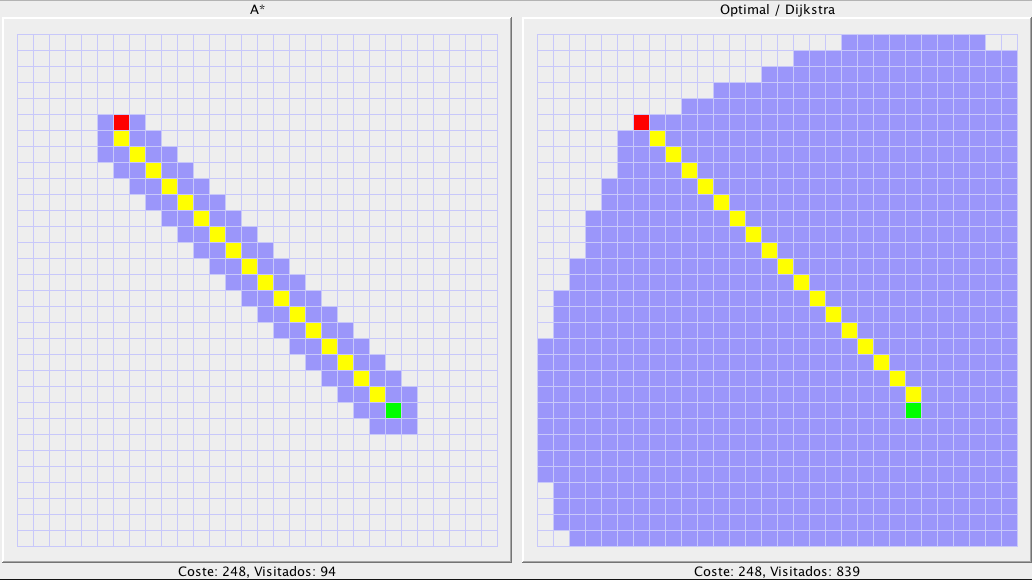
\includegraphics[width=\textwidth]{resources/versus1}
\end{figure}

En la figura 1 podemos ver un ejemplo comparativo entre los nodos visitados y el coste del camino en una matriz sin obstáculos, como no hay obstáculos y la heurística aplicada es válida el algoritmo A* siempre se acerca a la meta, mientras que el optimal se va expandiendo en forma circular, siendo el centro el nodo de inicio, por eso tiene que evaluar un número mucho mayor de nodos.

\begin{figure}[h!]
    \caption{Búsqueda con obstáculos aleatorios.}
    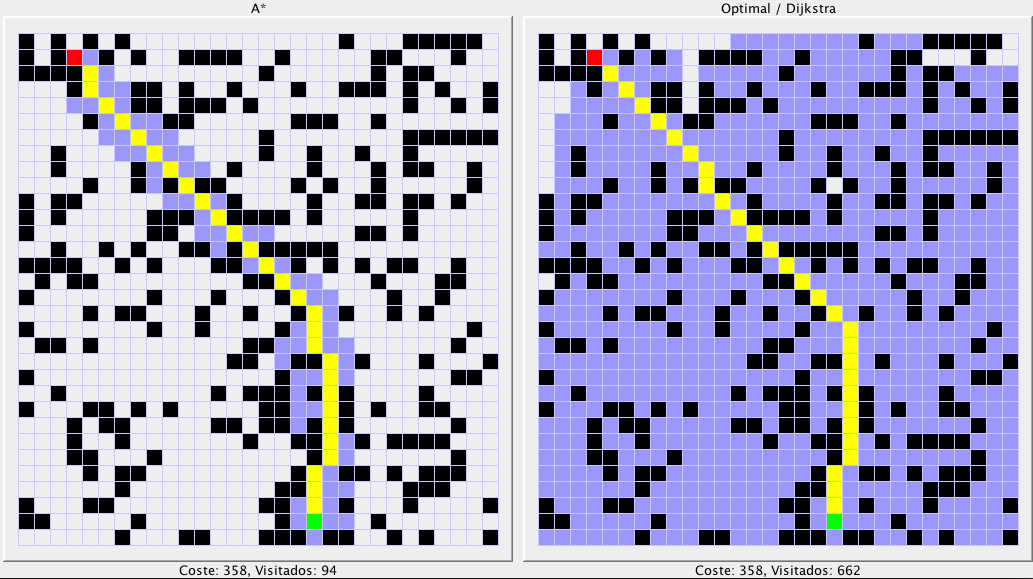
\includegraphics[width=\textwidth]{resources/versus2}
\end{figure}

\begin{figure}[h!]
    \caption{Búsqueda con obstáculos aleatorios.}
    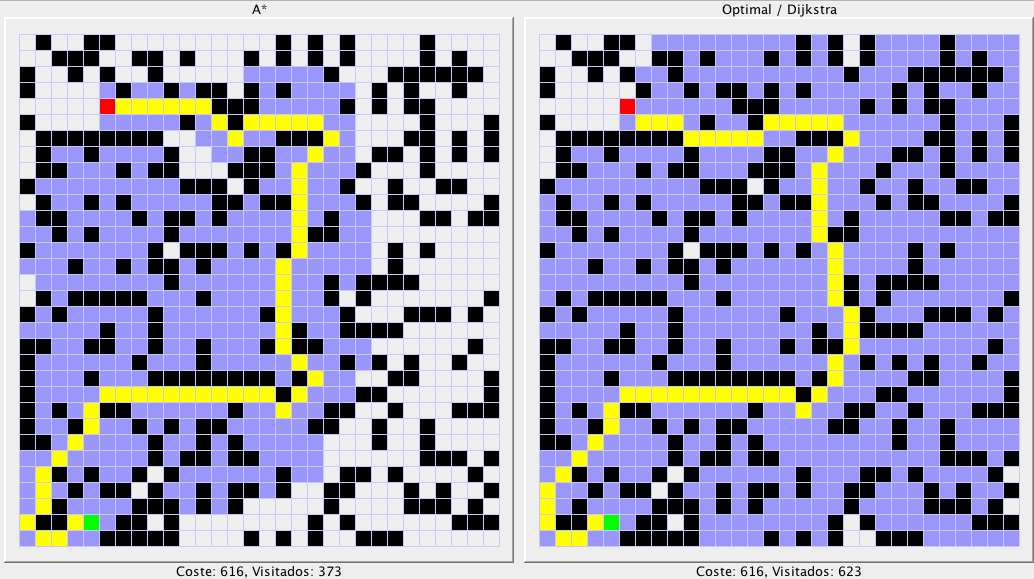
\includegraphics[width=\textwidth]{resources/versus3}
\end{figure}

Observando las figuras 2 y 3 podemos darnos cuenta de la diferencia y de cómo la cantidad y la posición de obstáculos ralentizan más a la búsqueda A*, ya que la heurística que mide la distancia no es tan eficaz. De una relación de 94 visitados por A* y 662 por Dijkstra / Optimal en la figura 2, que es bastante diferencia, pasamos a 363 visitados por A* y 623 visitados por Dijkstra / Optimal, cifras que comienzan a acercarse entre sí.

\begin{figure}[h!]
    \caption{Búsqueda con obstáculos específicos.}
    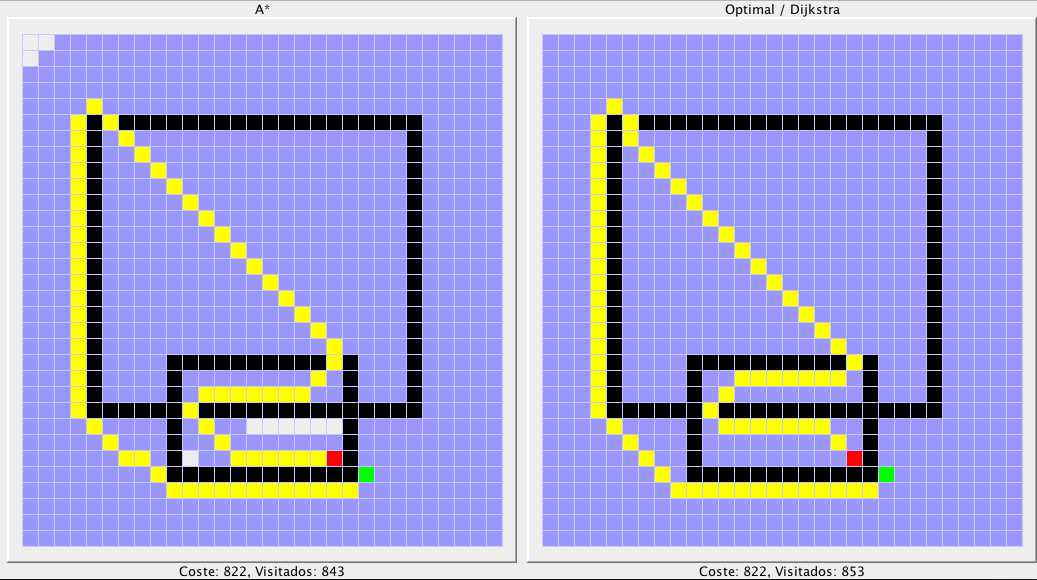
\includegraphics[width=\textwidth]{resources/versus4}
\end{figure}

Para terminar contemplaremos la figura 4, la cual tiene obstáculos específicos para engañar a la heurística, haciendo que la meta y el inicio estén muy cerca pero separados por un obstáculo, así podemos ver la poca diferencia que puede llegar a haber entre estos dos métodos, tan solo 10 nodos menos visitados por A* de un total de $\sim 850$ nodos.

\section{Conclusión}
Una vez vistos los ejemplos, podemos recoger las principales ideas expuestas. En general podemos decir que añadir métodos heurísticos a los algoritmos de resolución de caminos es una buena idea, ya que de forma general mejorará los resultados y en el peor caso más o menos igualaría a su equivalente no heurístico. Así hemos visto que el algoritmo de búsqueda A* se comporta mejor que el optimal en la mayoría de los ejemplos presentados, y en el peor caso iguala la cantidad de nodos a evaluar, añadiendo también el coste de evaluación de la heurística, que puede ser más o menos costoso. También podemos afirmar que en el caso de métodos de búsqueda a ciegas, el algoritmo de Dijkstra, aun siendo equivalente al optimal, es peor si hablamos tanto de complejidad espacial como temporal, por eso, a pesar del peso histórico de Dijkstra, se recomienda en general el uso de la búsqueda optimal.


\bibliographystyle{ieeetr}
\bibliography{ensayo}
\nocite{*}

\end{document}